%(BEGIN_QUESTION)
% Copyright 2010, Tony R. Kuphaldt, released under the Creative Commons Attribution License (v 1.0)
% This means you may do almost anything with this work of mine, so long as you give me proper credit

En trendskriver er koblet til en {\it strømtransformator}, som er klemt rundt en av effektlederne til trefasemotoren som driver en nytteheis. Når heisen løfter en last, omsettes motorens moment til linjestrøm, som måles og plottes av trendskriveren. Jo tyngre last som løftes, desto mer moment leverer motoren, og desto mer strøm trekker motoren.

$$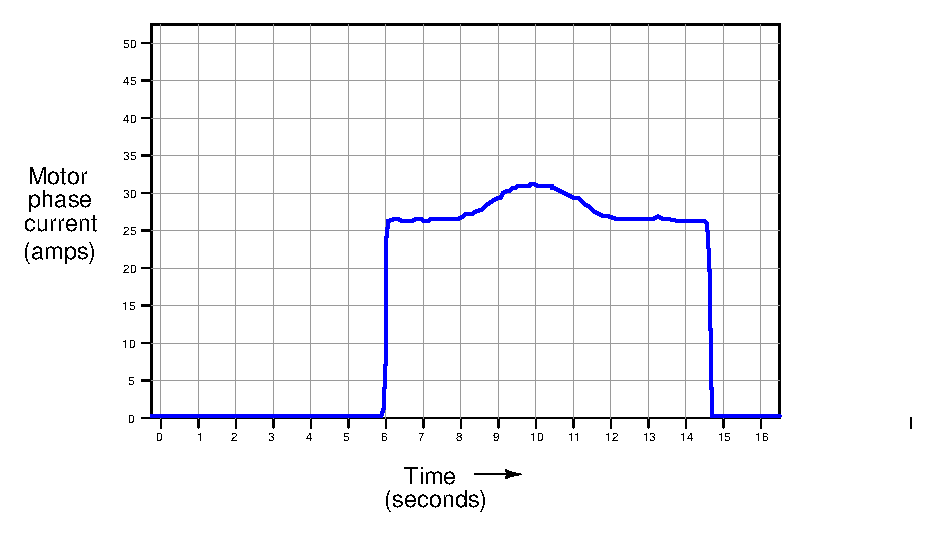
\includegraphics[width=15.5cm]{i01613x01.eps}$$

Beregn omtrent hvor mye {\it arbeid} denne heisen utfører (i joule), når du vet at effekten til en trefaset elektrisk motor er lik linjespenning (480 volt) ganger linjestrøm (plottet i grafen) ganger kvadratroten av 3, og også vet at én {\it watt} tilsvarer én {\it joule} arbeid utført per {\it sekund} (watt = joule per sekund):

$$P = U_{line} I_{line} \sqrt{3}$$

Forklar også betydningen av ``kulen'' som vises omtrent midt i heisens vandring. Hva antyder denne uvanlige formen om heisen?

\vfil 

\underbar{file i01613}
\eject
%(END_QUESTION)





%(BEGIN_ANSWER)

Dette er et vurdert spørsmål -- ingen svar eller hint er gitt!

%(END_ANSWER)





%(BEGIN_NOTES)

Måleenhetene i denne oppgaven forteller oss hvilken type kalkulusoperasjon vi må bruke. Siden motoreffekt (som kan tolkes direkte fra strømmen i grafen, gitt konstant linjespenning) måles i {\it watt}, som er {\it joule energi per sekund}, og tid naturlig måles i {\it sekunder}, må vi velge en matematisk operasjon som kansellerer tid (sekunder) og etterlater energi (joule). Vi må åpenbart bruke {\it multiplikasjon} for at sekunder skal kansellere joule per sekund og gi joule:

$$\left( {[\hbox{joule}] \over [\hbox{sekunder}]} \right) \left( {[\hbox{sekunder}] \over 1} \right)$$

Siden vi vet at multiplikasjon henger sammen med kalkulusoperasjonen {\it integrasjon}, kan vi fastslå at arbeid (energi) er integralet av effekt med hensyn på tid:

$$W = \int P \> dt$$

Den grafiske tolkningen av integrasjon er det geometriske arealet avgrenset av funksjonen. Derfor vil vi approksimere arealet mellom strømkurven og null. Én måte å gjøre dette på er å integrere strøm med hensyn på tid, som gir et resultat i enheten {\it ampere-sekunder}. Deretter kan vi multiplisere denne integrerte linjestrømmen med linjespenningen (480 VAC) og kvadratroten av 3 for å få et svar i watt-sekunder, som er det samme som joule:

$$[\hbox{Ampere-sekunder}] = \int I \> dt$$

$$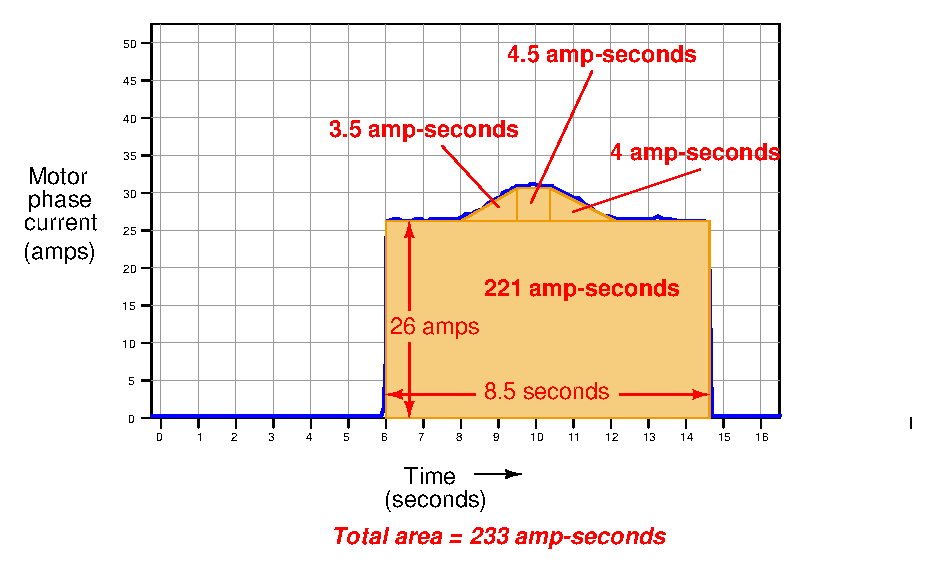
\includegraphics[width=15.5cm]{i01613x02.eps}$$

En integrert strømverdi på 233 ampere-sekunder multiplisert med $480 \sqrt{3}$ er omtrent lik 193{,}700 joule arbeid.

\vskip 10pt

``Kulen'' antyder mekanisk friksjon på ett punkt i heisens vandring. Dette er unormalt og bør undersøkes av relevant vedlikeholdspersonell.

%INDEX% Mathematics, calculus: integral (work)

%(END_NOTES)
